% Exam Template for UMTYMP and Math Department courses
%
% Using Philip Hirschhorn's exam.cls: http://www-math.mit.edu/~psh/#ExamCls
%
% run pdflatex on a finished exam at least three times to do the grading table on front page.
%
%%%%%%%%%%%%%%%%%%%%%%%%%%%%%%%%%%%%%%%%%%%%%%%%%%%%%%%%%%%%%%%%%%%%%%%%%%%%%%%%%%%%%%%%%%%%%%

% These lines can probably stay unchanged, although you can remove the last
% two packages if you're not making pictures with tikz.
\documentclass[11pt]{exam}
\RequirePackage{amssymb, amsfonts, amsmath, amsthm, latexsym, verbatim, xspace, setspace, mathrsfs, systeme, graphicx}
\RequirePackage{tikz, pgf, pgfplots}

% By default LaTeX uses large margins.  This doesn't work well on exams; problems
% end up in the "middle" of the page, reducing the amount of space for students
% to work on them.
\usepackage[margin=1in]{geometry}
\usepackage{textcomp}

\pgfplotsset{compat=1.15}
\usepgfplotslibrary{fillbetween}
\usetikzlibrary{plotmarks}
\usetikzlibrary{arrows}
\usetikzlibrary{calc}

% Here's where you edit the Class, Exam, Date, etc.
\newcommand{\class}{College Algebra}
\newcommand{\term}{Fall 2022}
\newcommand{\examnum}{Exam Two}
\newcommand{\examdate}{10/17/22}
\newcommand{\timelimit}{80 Minutes}

% For an exam, single spacing is most appropriate
\singlespacing
% \onehalfspacing
% \doublespacing

% For an exam, we generally want to turn off paragraph indentation
\parindent 0ex

\begin{document} 

% These commands set up the running header on the top of the exam pages
\pagestyle{head}
\firstpageheader{}{}{}
\runningheader{\class}{\examnum\ - Page \thepage\ of \numpages}{\examdate}
\runningheadrule

\begin{flushright}
\begin{tabular}{p{2.8in} r l}
\textbf{\class} & \textbf{Your Name:} & \makebox[2in]{\hrulefill}\\
\textbf{\term} &&\\
\textbf{\examnum} & \textbf{Instructor:} & \makebox[2in]{\hrulefill}\\
\textbf{\examdate} &&\\
\textbf{Time Limit: \timelimit} 
\end{tabular}\\
\end{flushright}
\rule[1ex]{\textwidth}{.1pt}


This exam contains \numpages\ pages (including this cover page) and
\numquestions\ problems.  Check to see if any pages are missing.  Enter
all requested information on the top of this page, and put your initials
on the top of every page, in case the pages become separated.\\

You may \textit{not} use your books, notes, or \textbf{any calculator} on this exam.\\

You are required to show your work on each problem on this exam.  The following rules apply:\\

\begin{minipage}[t]{3.7in}
\vspace{0pt}
\begin{itemize}

\item \textbf{Organize your work}, in a reasonably neat and coherent way, in
the space provided. Work scattered all over the page without a clear ordering will 
receive very little credit.  

\item \textbf{Box your final answer} and label the solution with the appropriate variables (if applicable).

\item \textbf{Simplify your final answer}. A correct answer, written in an unsimplified way, will receive less than full credit. All fractions must be written such that the numerator and denominator share no common factors.

\item Do not leave a question blank. You will not be penalized for incorrect work, and partial answers may receive partial credit.
\end{itemize}

Do not write in the table to the right.
\end{minipage}
\hfill
\begin{minipage}[t]{2.3in}
\vspace{0pt}
%\cellwidth{3em}
\gradetablestretch{2}
\vqword{Problem}
\addpoints % required here by exam.cls, even though questions haven't started yet.	
\gradetable[v]%[pages]  % Use [pages] to have grading table by page instead of question

\end{minipage}
\newpage % End of cover page

%%%%%%%%%%%%%%%%%%%%%%%%%%%%%%%%%%%%%%%%%%%%%%%%%%%%%%%%%%%%%%%%%%%%%%%%%%%%%%%%%%%%%
%
% See http://www-math.mit.edu/~psh/#ExamCls for full documentation, but the questions
% below give an idea of how to write questions [with parts] and have the points
% tracked automatically on the cover page.
%
%
%%%%%%%%%%%%%%%%%%%%%%%%%%%%%%%%%%%%%%%%%%%%%%%%%%%%%%%%%%%%%%%%%%%%%%%%%%%%%%%%%%%%%

\begin{questions}

% Easy Points

\question[5] Write your name and the name of the instructor on page one. 
\question[5] How many points are needed to uniquely determine a line?

\addpoints
\question Use the coordinate grid to do the following:
\begin{center}
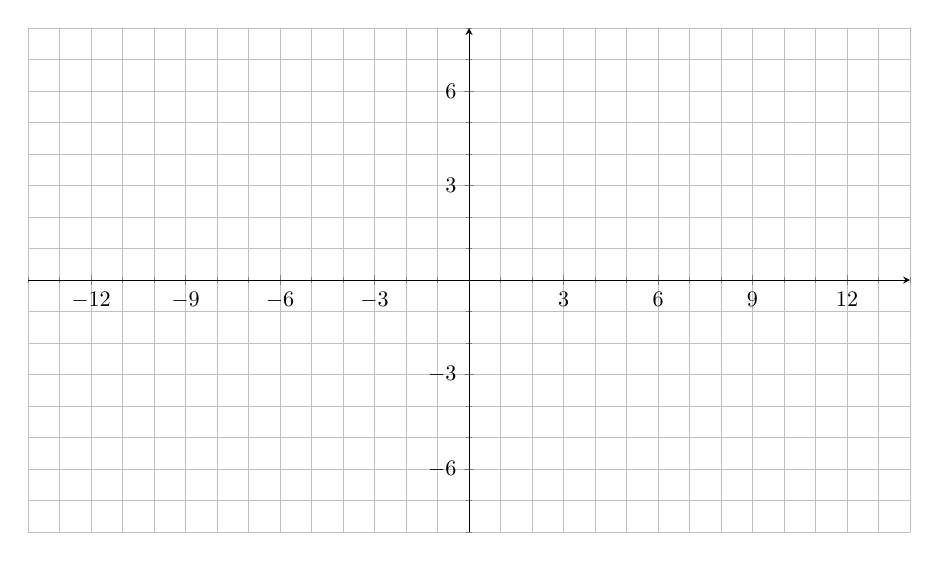
\begin{tikzpicture}[scale=0.8]

\begin{axis}[axis lines=middle,grid=both,
            xtick distance=3,ytick distance=3,minor tick num=2,
            x=0.5cm,y=0.5cm,xmin=-14,xmax=14,ymin=-8,ymax=8]
% no plots to draw ... just empty grid with axes
\end{axis}
\end{tikzpicture}
\end{center}

\begin{parts}
\part[2] Label the Four Quadrants
\part[2] Draw and Label the Points: \quad $P(0,0)$ \quad $Q(2,-4)$ \quad $R(-12,5)$
\part[1] Draw the Line through the Points: \quad $A(-6, -3)$ \quad $B(9,4)$
\end{parts}

\addpoints
\question Find the Slope Between the Two Points:
\begin{parts}
\part[2] $$A(9,10) \text{\quad} B(6,2)$$
\vfill
\part[2] $$E(-2,4) \text{\quad} F(6,4)$$
\vfill
\part[2] $$I(2,8) \text{\quad} J(7,2)$$
\vfill
\part[2] $$M(-8,-3) \text{\quad} N(-2,-11)$$
\vfill
\part[2] $$P(a,b) \text{\quad} Q(c,d)$$
\vfill
\end{parts}

% Linear Equations

\newpage

\question[5] Write the Equations:
\begin{parts}
\part Standard Form
\part Slope-Intercept
\part Point-Slope
\end{parts}

\addpoints
\question Find the Equation for the Line Between the Points in the Given Form:
\begin{parts}
\part[5]  Point-Slope: $$A(7,11) \text{\quad} B(8,14)$$
\vfill
\part[5] Slope-Intercept: $$E(0,0) \text{\quad} F(-3,-5)$$
\vfill
\part[5] Your Choice: $$I(-5,3) \text{\quad} J(1,3)$$
\vfill
\part[5] Standard Form: $$M(5,-1) \text{\quad} N(5,12)$$
\vfill
\part[5] Point-Slope: $$X(a,a) \text{\quad} Y(b,b)$$
\vfill
\end{parts}

% Matrix Stuff
\newpage

\addpoints
\question Solve the System of Linear Equations Using the Given Method:
\begin{parts}
\part[10] Substitution: $$\begin{bmatrix}
                x - 5y = 7 \\
                4x + 9y = 28
                \end{bmatrix}$$
\vfill
\part[10] Elimination: $$\begin{bmatrix}
                x - 4y = 29 \\
                3x + 2y = -11 
                \end{bmatrix}$$
\vfill
\part[5] Your Choice: $$\begin{bmatrix}
                5x - 2y = 1 \\
                10x - 4y = 7
                \end{bmatrix}$$
\vfill
\part[5] Your Choice: $$\begin{bmatrix}
                x = \frac{1}{2} y - 3 \\
                5x - y = 9
                \end{bmatrix}$$
\vfill
\end{parts}

% Polynomials

\newpage

\addpoints
\question Simplify:
\begin{parts}
\part[5] $$ (8x^{4} - 3x^2 + 5x + 2) + (5x^4 + 11x^3 + 10x^2 + 1) $$
\vfill
\part[5] $$ (3x^3 + 12x^2 - 4x + 1) - (5x^2 + 3x + 23) $$
\vfill
\part[5] $$ (5x - 1) \cdot (x^2 + 7x + 10) $$
\vfill
\part[5] $$ \frac{x^{3} + 8}{x + 2} $$
\vfill
\part[5] $$ \left( \frac{-52x^6y^5z^4}{13x^2y^5z^7}\right)^{2} $$
\vfill
\end{parts}

\end{questions}
\end{document}
